\section{Related Work}
\label{sec:related}

\subsection{Software Attestation Overview}

The security of systems that employ trusted processors hinges on
\textit{software attestation}. The software running inside an \textit{isolated
container} established by trusted hardware can ask the hardware to sign a
small piece of \textit{attestation data}, producing an
\textit{attestation signature}. Asides from the attestation data, the signature
includes a \textit{measurement} that uniquely identifies the software inside
the container. Therefore, an attestation signature can be used to convince a
\textit{verifier} that the attestation data was produced by a specific piece
of software, which is hosted inside a container that is isolated from outside
interference by trusted hardware.

Each hardware platforms discussed in this section uses a slightly different
software attestation scheme. Platforms differ by the amount of software that
executes inside an isolated container, by the isolation guarantees provided to
the software inside a container, and by the process used to obtain a
container's measurement. The threat model and security properties of each
trusted hardware platform follow directly from the design choices outlined
above, so a good understanding of attestation is a prerequisite to discussing
the differences between existing platforms.

Software attestation can be used to authenticate one party in a key exchange
protocol. The resulting protocol can assure a verifier that it is communicating
over a secure channel with a specific piece of software, hosted inside an
isolated container created by trusted hardware. The next paragraph outlines the
augmented protocol, using Diffie-Hellman Key Exchange (DKE)
\cite{diffie1976keyexchange} as an example key exchange protocol.

The verifier starts executing the key exchange protocol, and sends the first
message, $g^{A}$, to the software inside the secure container. The software
inside the container produces the second key exchange message, $g^{B}$, and
asks the trusted hardware to attest the cryptographic hash of both key exchange
messages, $h(g^{A} || g^{B})$. The verifier receives the second key exchange
and attestation signature, and authenticates the software inside the secure
container by checking all the signatures along the \textit{attestation chain}
of trust shown in Figure~\ref{fig:generic_attestation_chain}.

\begin{figure}[hbt]
  \centering
  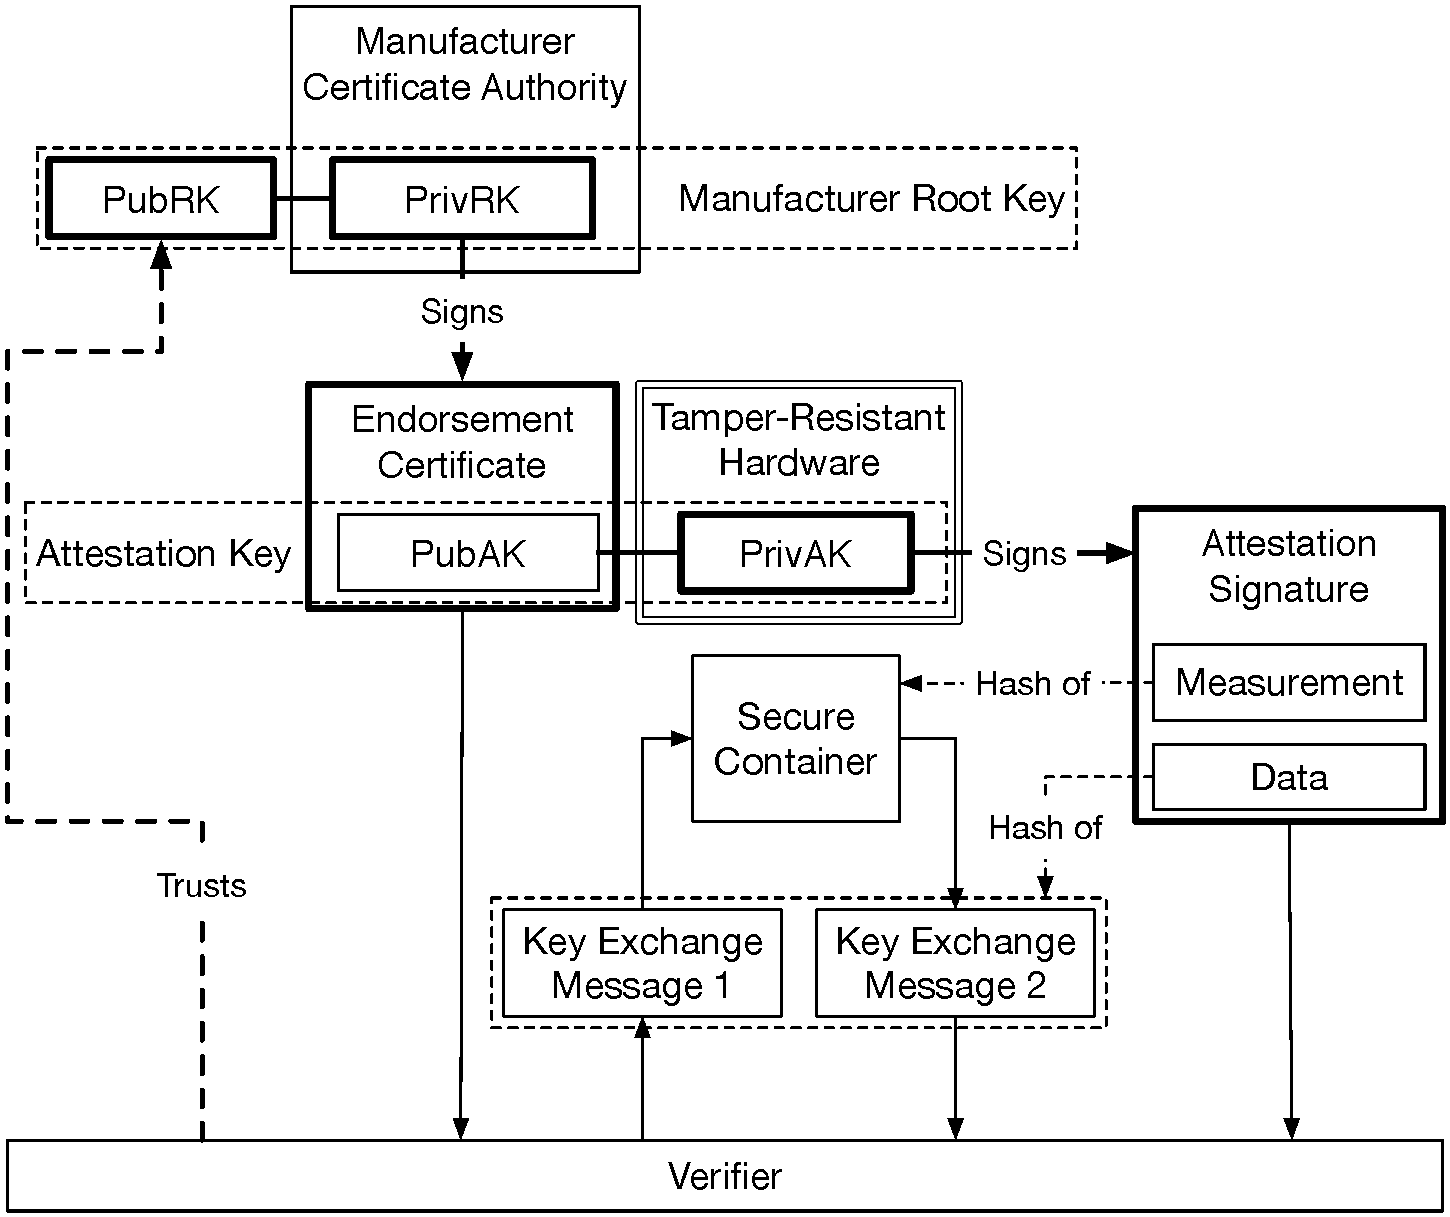
\includegraphics[width=85mm]{figures/generic_attestation_chain.pdf}
  \caption{
    The chain of trust in software attestation. The root of trust is a
    manufacturer key, which produces an endorsement certificate for the secure
    processor's attestation key. The processor signs the attestation
    certificate, which contains a cryptographic hash of the container, and a
    message produced by the software inside the container.
  }
  \label{fig:generic_attestation_chain}
\end{figure}

The chain of trust used in software attestation is rooted at a signing key
owned by the hardware manufacturer, which must be trusted by the verifier. The
manufacturer acts as a Certificate Authority (CA), and provisions each secure
processor that it produces with a unique \textit{attestation key}, which is
used to produce \textit{attestation signatures}. The manufacturer also
generates an \textit{endorsement certificate} for each secure processor,
by signing the public part of the processor's attestation key with the
manufacturer \textit{root key}. When the verifier receives a valid endorsement
certificate signed by a manufacturer key that it trusts, the verifier is
assured that the private part of the attestation key in the certificate is
stored in tamper-resistant hardware, and is only used for producing attestation
signatures, under the rules set by the trusted manufacturer.

A secure processor identifies each isolated container by storing a
cryptographic hash of the code executed inside the container. When the
processor is asked to sign a piece of attestation data, it uses the
cryptographic hash associated with the container as the measurement in the
attestation signature. After a verifier validates the processor's attestation
key using its endorsement certificate, the verifier ensures that the signature
is valid, and that the measurement in the signature belongs to the software
that it expects to communicate with. Having checked all the links in the
attestation chain, the verifier has authenticated the other party in the key
exchange, and is assured that it now shares a secret with the software that it
expects, running in an isolated container on hardware that it trusts.


\subsection{Secure Processors in the Industry}

The Trusted Platform Module (TPM) \cite{grawrock2003tpm} introduced the
software attestation model described above, and was the first widely deployed
. The
TPM model relies on a tamper-resistant chip that is dedicated to storing the
attestation key and using it to perform software attestation. The following
paragraphs highlight the issues in the TPM design, in order to facilitate an
understanding of its successors.

The TPM design provides one isolation container, covering all the software
running on the computer that has the TPM chip. It follows that the measurement
included in an attestation signature covers the entire OS kernel and all the
kernel modules, such as device drivers. However, commercial computers use a
wide diversity of devices, and their system software is updated at an
ever-increasing pace, so it is impossible to maintain a list of acceptable
measurement hashes corresponding to a piece of trusted software. Due to this
issue, the TPM's software attestation is not used in many security systems,
despite its wide deployment.

The TPM design is technically not vulnerable to any software attacks, because
it trusts all the software on the computer. However, a TPM-based system is
vulnerable to an attacker who has physical access to the machine, as the TPM
chip does not provide any isolation for the software on the computer.
Furthermore, the TPM chip receives the software measurements from the CPU,
so TPM-based systems are vulnerable to attackers who can tap the communication
bus between the CPU and the TPM.

Last, the TPM's design relies on the software running on the CPU to report its
own cryptographic hash. The TPM chip resets the measurements stored in Platform
Configuration Registers (PCRs) when the computer is rebooted. Then, the TPM
expects the software at each boot stage to cryptographically hash the software
at the next stage, and send the hash to the TPM. The TPM updates the PCRs to
incorporate the new hashes it receives, as shown in
Figure~\ref{fig:tpm_measurement}. Most importantly, the PCR value at any point
reflects all the software hashes received by the TPM up to that point. This
makes it impossible for software that has been measured to ``remove'' itself
from the measurement.

\begin{figure}[hbt]
  \centering
  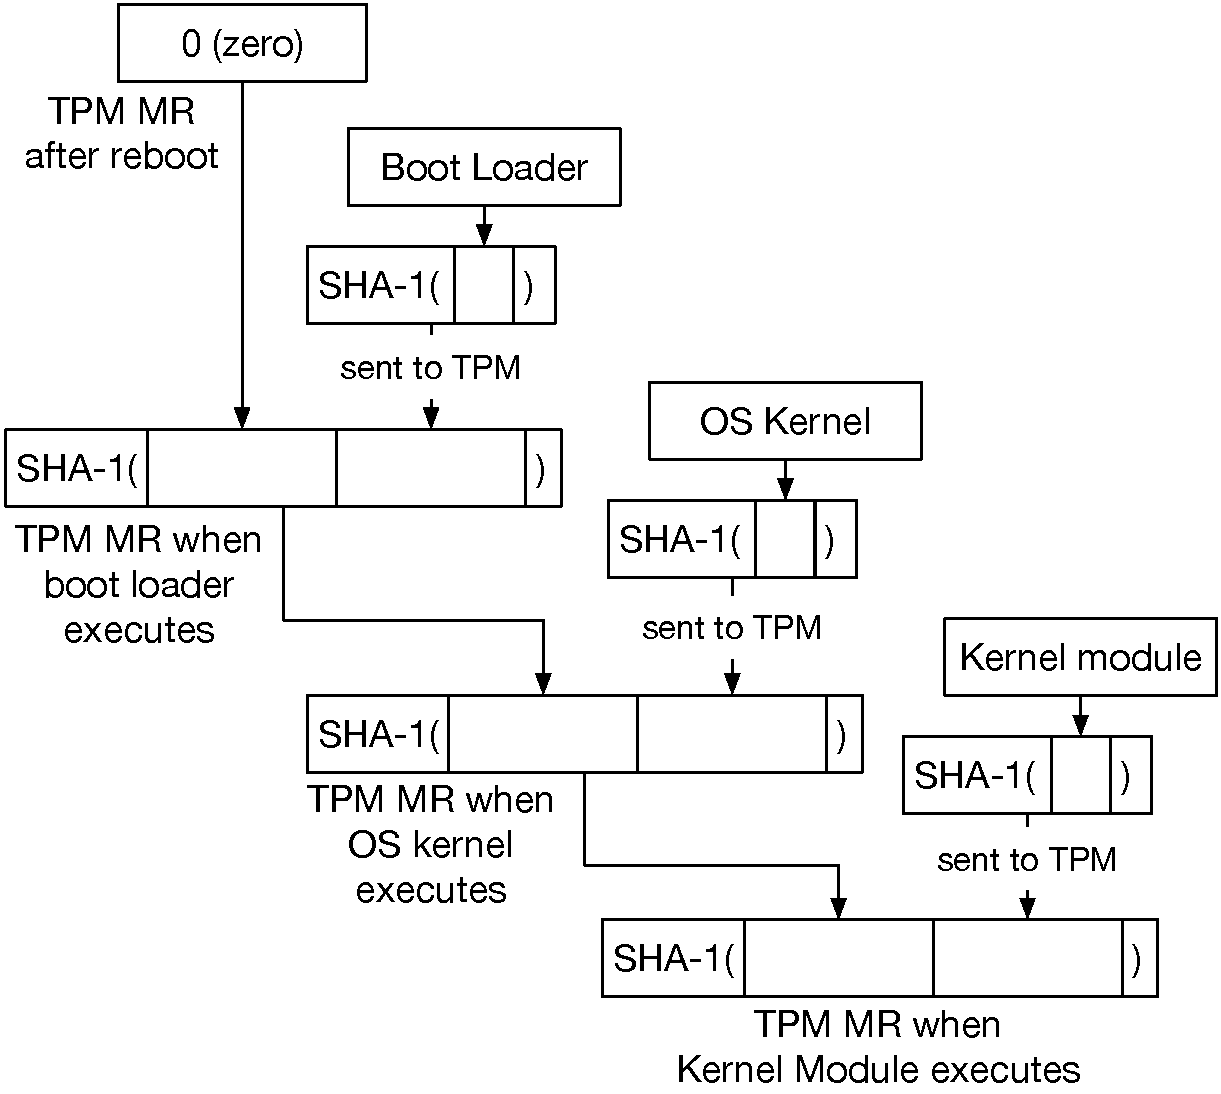
\includegraphics[width=85mm]{figures/tpm_measurement.pdf}
  \caption{
    The measurement stored in a TPM platform configuration register (PCR). The
    PCR is reset when the system reboots. The software at every boot stage
    hashes the next boot stage, and sends the hash to the TPM. The PCR's new
    value incorporates both the old PCR value, and the new softare hash.
  }
  \label{fig:tpm_measurement}
\end{figure}

Unfortunately, the security of the whole measurement scheme hinges on the
requirement that the first hash sent to the TPM must reflect the software that
runs in the first boot stage. The TPM threat model explicitly acknowledges this
issue, and assumes that the firmware responsible for loading the first stage
bootloader is securely embedded in the motherboard. However, virtually every
TPM-enabled computer stores its firmware in a flash memory chip that can be
re-programmed in software (\S~\ref{sec:motherboard}), so the TPM's measurement
can be subverted by an attacker that can reflash the computer's firmware
\cite{butterworth2013bios}.

On very recent Intel processors, the attack described above can be defeated by
having the initialization microcode (\S~\ref{sec:microcode_sec}) hash the
computer's firmware (specifically, the PEI code in UEFI \cite{forum2015uefi}
firwmare) and communicate the hash to the TPM chip. This is marketed as the
Measured Boot feature of Intel's Boot Guard \cite{ruan2014intelme}.

Sadly, most computer manufacturers use Verified Boot (also known as ``secure
boot'') instead of Measured Boot (also known as ``trusted boot''). Verified
Boot means that the processor's microcode only boots into PEI firmware that
contains a signature produced by a key burned into the chip's e-fuses. Verified
Boot does not impact the measurements stored on the TPM, so it does not improve
the security of software attestation.


\subsection{The XOM Architecture}

The execute-only memory (XOM) architecture \cite{lie2000xom} introduced the
approach of having sensitive code and data execute in isolated containers
managed by untrusted host software. XOM outlined the mechanisms needed to
isolate a container's data from its untrusted software environment, such as
saving the register state to a protected memory area before servicing an
interrupt.

XOM supports multiple containers by tagging every cache line with the
identifier of the container owning it, and ensures isolation by disallowing
memory accesses to cache lines that don't match the current container's
identifier. The operating system and the untrusted applications are considered
to belong to a container with a null identifier.

XOM also introduced the integration of encryption and HMAC funcationality in
the processor's memory controller to protect container memory from physical
attacks on DRAM. The encryption and HMAC functionality is used for all cache
line evictions and fetches, and the ECC bits in DRAM chips are repurposed to
store HMAC values.

XOM's design cannot guarantee DRAM freshness, so the software in its containers
is vulnerable to physical replay attacks. Furthermore, XOM does not protect a
container's memory access patterns, meaning that any piece of malicious
software can perform cache timing attacks against the software in a container.
Last, XOM containers are destroyed when they encounter hardware exceptions,
such as including page faults, so XOM does not support paging.

XOM pre-dates the attestation scheme described above, and relies on a modified
software distribution scheme instead. Each container's contents is encrypted
with a symmetric key, which also serves as the container's identity. The
symmetric key, in turn, is encrypted with the public key of each CPU that is
trusted to run the container. A container's author can be assured that the
container is running on trusted software by embedding a secret into the
encrypted container data, and using it to authenticate the container. While
conceptually simpler than software attestation, this scheme does not allow the
container author to vet the container's software environment.


\subsection{The Aegis Secure Processor}

The Aegis secure processor \cite{suh2003aegis} argued that Physically
Uncloneable Functions (PUFs) \cite{gassend2002puf} can be used to endow a
secure processor with a tamper-resistant private key, which is required for
software attestation. PUFs do not have the fabrication process drawbacks of
EEPROM, and are significantly more resilient to physical attacks than e-fuses.
Aegis relies on a security kernel in the operating system to isolate
containers, and includes the kernel's cryptographic hash in the measurement
reported by the software attestation signature.

Aegis relies on a trusted security kernel to isolate each container from the
other software on the computer by configuring the page tables used in address
translation. As the security kernel is a part of the \textit{trusted code base}
(TCB), its cryptographic hash is included in the software attestation
measurement.

The Aegis memory controller encrypts the cache lines in one memory range, and
HMACs the cache lines in one other memory range. The two memory ranges can
overlap, and are configurable by the security kernel. Thanks to the two ranges,
the memory controller can avoid the latency overhead of cryptographic
operations for the DRAM outside containers.

Aegis uses a Merkle tree construction \cite{gassend2003merkle} to guarantee
DRAM freshness, so it is not vulnerable to physical replay attacks. The latency
overhead of the Merkle tree is greatly reduced by augmenting the L2 cache with
the tree nodes for the cache lines. Unlike XOM, Aegis does not tag its cache
lines with container identifiers, as the page tables and the configurable
memory ranges are sufficient for software and hardware isolation.

Aegis' security kernel allows the OS to page out container memory, but verifies
the correctness of the paging operations. The security kernel uses the same
encryption and Merkle tree algorithms as the memory controller to guarantee the
privacy and integrity of the container pages that are swapped out from DRAM.
As the OS is free to page out container memory, it can learn a containter's
memory access patterns, at page granularity. Aegis containers are also
vulnerable to cache timing attacks.



